%% =====================================================================
\section{Background}\label{sec:background}
%% =====================================================================

\subsection{The N-Queens problem}
We index the cells by $(i,j)$ with $0\le i,j<N$. A set $Q$ of $N$ cells is a solution if, for every two distinct cells $(i,j),(i',j')\in Q$:
\begin{equation}
  i\neq i',\qquad j\neq j',\qquad i-j\neq i'-j',\qquad i+j\neq i'+j'.
\end{equation}
So every \textbf{row} and every \textbf{column} contains \emph{exactly one} queen, and every \textbf{diagonal} contains \emph{at most one} queen. (There are $2N-1$ diagonals in each direction but only $N$ queens, so ``exactly one'' on diagonals would be unsatisfiable.) The number of solutions for $N=2,\dots,9$ is $0,0,2,10,4,40,92,352$; we use these values to validate our encodings (Section~\ref{sec:correct}). Fig.~\ref{fig:board} shows one solution for $N=8$ and the four lines that pass through one cell.

\begin{figure}[pos=htbp]
\centering
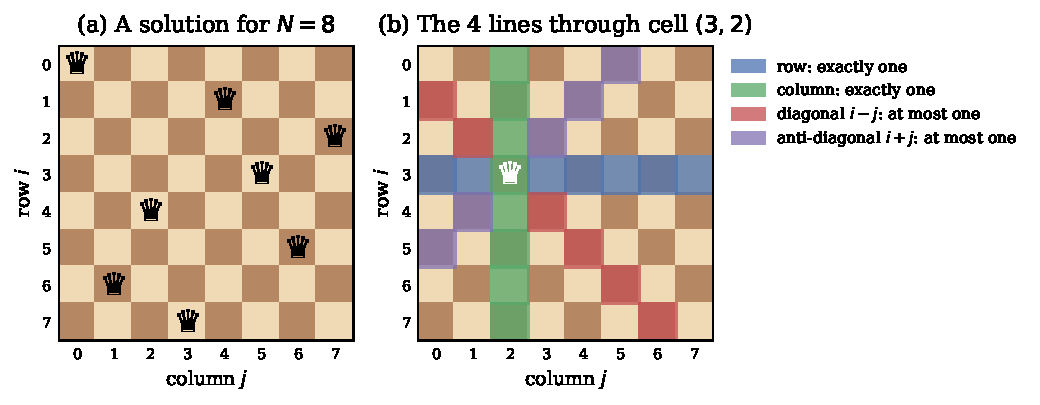
\includegraphics[width=0.95\linewidth]{figures/board.pdf}
\caption{(a) One solution for $N=8$ (the queen of row $i$ is in column $0,4,7,5,2,6,1,3$). (b) Each cell lies on one row, one column, one diagonal and one anti-diagonal. Rows and columns must contain exactly one queen; diagonals at most one.}\label{fig:board}
\end{figure}

\paragraph{Lines.} We call every row, column, diagonal ($i-j=d$) and anti-diagonal ($i+j=s$) a \emph{line}. Each direction has $2N-1$ diagonals, of which the two corner diagonals have length 1 and impose no constraint. Hence there are
\begin{equation}\label{eq:lines}
  \underbrace{2N}_{\text{rows+columns}} + \underbrace{2(2N-3)}_{\text{diagonals, length}\ge2} = 6N-6 \text{ lines, of total length } 4N^2-4.
\end{equation}
All three paradigms below model exactly these $6N-6$ lines; they only differ in \emph{how} a line constraint is expressed.

%% ---------------------------------------------------------------------
\subsection{Propositional logic and SAT}
A \emph{literal} is a Boolean variable $x$ or its negation $\neg x$. A \emph{clause} is a disjunction (OR) of literals, and a formula in \emph{conjunctive normal form} (CNF) is a conjunction (AND) of clauses. The SAT problem asks whether a CNF formula has an assignment that makes every clause true; a solver answers SAT (with a model) or UNSAT. Solvers read the DIMACS format, where each clause is a line of signed integers ending with 0. For example, ``at most one of $x_1,x_2,x_3$'' in pairwise form is
\begin{center}
\texttt{p cnf 3 3}\qquad \texttt{-1 -2 0}\qquad \texttt{-1 -3 0}\qquad \texttt{-2 -3 0}
\end{center}
Every formula has an equivalent CNF, but direct conversion can grow exponentially. Introducing \emph{auxiliary variables} (as in the Tseitin transformation) keeps the CNF small. The resulting formula is \emph{equisatisfiable}: it is satisfiable exactly when the original one is, and every model restricted to the original variables is a model of the original formula. All AMO encodings in Section~\ref{sec:amo} except pairwise use this idea.

%% ---------------------------------------------------------------------
\subsection{How CDCL solvers work}\label{sec:cdcl}

\paragraph{DPLL and unit propagation.}
Classic DPLL search repeats three steps: \emph{decide} (assign a value to a free variable), \emph{unit propagation} (UP) and \emph{backtrack} on conflict. A clause is \emph{unit} when all its literals but one are false; the last literal must then be true. UP applies this rule until no unit clause is left or a clause becomes fully false (a \emph{conflict}). UP typically takes more than 90\% of the run time of a solver. This is why the shape of an encoding (how many clauses each assignment touches, and how long the chains of implications are) matters so much in practice.

\paragraph{Conflict-driven clause learning.}
CDCL~\cite{marques2009} extends DPLL with the following components (Algorithm~\ref{alg:cdcl}):
\begin{itemize}
  \item \textbf{Decision levels and implication graph.} Every decision opens a new level. Each propagated literal stores the clause that implied it (its \emph{reason}).
  \item \textbf{Conflict analysis (1UIP).} On a conflict the solver resolves the conflicting clause with reason clauses backwards until exactly one literal of the current level remains (the \emph{first unique implication point}). The result is a new \emph{learned clause} that is implied by the formula.
  \item \textbf{Non-chronological backjumping.} The solver jumps back to the second-highest level in the learned clause, where the clause becomes unit and immediately propagates.
  \item \textbf{Heuristics.} VSIDS-style branching prefers variables that appeared in recent conflicts; \emph{phase saving} reuses a variable's last value; \emph{restarts} restart the search while keeping learned clauses; \emph{clause deletion} removes learned clauses of low quality, e.g.\ measured by literal block distance (LBD)~\cite{audemard2009}.
  \item \textbf{Two watched literals}~\cite{moskewicz2001}: each clause is only visited when one of its two watched literals becomes false, which makes UP fast on large formulas.
\end{itemize}

\begin{algorithm}[htbp]
\caption{CDCL (simplified)}\label{alg:cdcl}
\begin{algorithmic}[1]
\Require CNF formula $F$
\State $level \gets 0$
\Loop
  \State $conflict \gets \textsc{UnitPropagate}()$
  \If{$conflict$}
    \If{$level = 0$} \Return UNSAT \EndIf
    \State $(C, b) \gets \textsc{AnalyzeConflict}()$ \Comment{1UIP learned clause $C$, backjump level $b$}
    \State $F \gets F \cup \{C\}$;\; \textsc{Backjump}$(b)$;\; $level \gets b$
  \ElsIf{all variables are assigned}
    \State \Return SAT
  \Else
    \State occasionally \textsc{Restart}() and \textsc{ReduceLearnedClauses}()
    \State $\ell \gets$ \textsc{Decide}() \Comment{VSIDS + phase saving}
    \State $level \gets level+1$; assign $\ell$
  \EndIf
\EndLoop
\end{algorithmic}
\end{algorithm}

\paragraph{Worked example: CDCL on 4-Queens.}
Fig.~\ref{fig:cdcl} follows CDCL on $N=4$ with the pairwise encoding.
\begin{enumerate}
  \item[(a)] The solver decides $x_{00}=1$ at level 1. UP on the AMO clauses falsifies the rest of row 0, column 0 and the main diagonal. No ALO clause becomes unit yet.
  \item[(b)] It decides $x_{12}=1$ at level 2. UP falsifies $x_{21}$ (anti-diagonal) and $x_{23}$ (diagonal), while $x_{20},x_{22}$ were already false at level 1. The ALO clause of row 2, $(x_{20}\vee x_{21}\vee x_{22}\vee x_{23})$, is now false: a conflict. (Depending on propagation order the conflict may be detected on another clause first.)
  \item[(c)] Resolving the conflicting clause with the reasons $(\neg x_{12}\vee\neg x_{21})$ and $(\neg x_{12}\vee\neg x_{23})$ yields the 1UIP clause $(x_{20}\vee x_{22}\vee\neg x_{12})$. The solver backjumps to level 1, where this clause is unit and forces $x_{12}=0$. UP then forces $x_{13}=1$ (row 1 has no other free cell) and $x_{21}=1$ (row 2), after which row 3 has no free cell: a new conflict at level 1.
  \item[(d)] Every path in the implication graph of this conflict starts at the decision $x_{00}$, so analysis learns the unit clause $(\neg x_{00})$: \emph{no 4-Queens solution has a queen in a corner}. The solver continues at level 0 and soon finds a solution.
\end{enumerate}
The example shows how a CDCL solver turns a failed branch into a reusable fact (a learned clause), instead of re-discovering the same conflict in other branches as plain backtracking would.

\begin{figure}[pos=htbp]
\centering
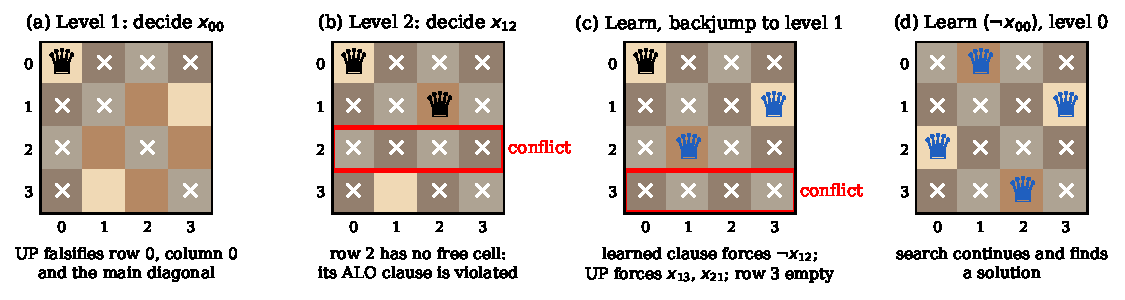
\includegraphics[width=\linewidth]{figures/cdcl_example.pdf}
\caption{CDCL on 4-Queens (pairwise encoding). Black queens are decisions, blue queens are forced by unit propagation, grey cells are falsified by unit propagation, and red frames mark the clause that caused the conflict.}\label{fig:cdcl}
\end{figure}

\paragraph{Solvers used.}
All solvers used here are CDCL solvers, but they differ in heuristics and in how much \emph{inprocessing} (formula simplification during search) they perform (Table~\ref{tab:solverfeat}). We use them through PySAT~\cite{ignatiev2018}, except CryptoMiniSat~\cite{soos2009}, which we call through its own Python binding.

\begin{table}[pos=htbp]
\caption{Main characteristics of the SAT solvers used.}\label{tab:solverfeat}
\centering\small
\begin{tabular}{lp{11.2cm}}
\toprule
Solver & Main characteristics \\
\midrule
MiniSat 2.2~\cite{een2003} & Compact reference CDCL solver: VSIDS, 1UIP learning with clause minimisation, Luby restarts, phase saving. Little extra machinery. \\
Glucose 4 & MiniSat-based; ranks learned clauses by LBD, deletes low-quality clauses aggressively and restarts dynamically based on recent LBD values~\cite{audemard2009}. \\
CaDiCaL 1.5.3 / 1.9.5~\cite{biere2020} & Modern solver with heavy inprocessing (vivification, subsumption, variable elimination, probing). Alternates between a ``focused'' mode (frequent restarts) and a ``stable'' mode (rare restarts). \\
Kissat 4.0.4~\cite{biere2020} & Re-implementation of CaDiCaL's ideas in C with compact data structures; winner of several recent SAT competitions. \\
Lingeling & Predecessor of CaDiCaL by the same author; also inprocessing-heavy. \\
MapleChrono & Maple family (learning-rate-based branching~\cite{liang2016}) combined with chronological backtracking~\cite{nadel2018}; tuned for hard competition instances. \\
CryptoMiniSat 5~\cite{soos2009} & Detects XOR constraints and reasons about them with Gaussian elimination, plus inprocessing. \\
\bottomrule
\end{tabular}
\end{table}

%% ---------------------------------------------------------------------
\subsection{AMO and ALO encodings}\label{sec:amo}
For Boolean variables $x_1,\dots,x_m$, the \textbf{at-least-one} (ALO) constraint is the single clause $x_1\vee\dots\vee x_m$, and ``exactly one'' = ALO + AMO. The \textbf{at-most-one} (AMO) constraint can be encoded in many ways. We implement five; the precise rules below are those of our implementation (they reproduce all counts in Table~\ref{tab:size} exactly).

\begin{itemize}
  \item \textbf{Pairwise (binomial).} For every pair $i<j$ add $(\neg x_i\vee\neg x_j)$. No auxiliary variables, $\binom{m}{2}$ clauses.
  \item \textbf{Binary}~\cite{frisch2010}. Add $k=\lceil\log_2 m\rceil$ variables $y_1,\dots,y_k$. Variable $x_i$ ($i=1..m$) receives the $k$-bit code of $i-1$, and for each bit $j$ we add $(\neg x_i\vee y_j)$ if the bit is 1 and $(\neg x_i\vee\neg y_j)$ if it is 0. Thus a true $x_i$ ``writes'' its code into $y$. In total $m\lceil\log_2 m\rceil$ clauses.
  \item \textbf{Sequential counter}~\cite{sinz2005}. Add $m-1$ variables $s_i$ meaning ``some of $x_1,\dots,x_i$ is true'': $(\neg x_1\vee s_1)$; for $1<i<m$: $(\neg x_i\vee s_i)$, $(\neg s_{i-1}\vee s_i)$, $(\neg s_{i-1}\vee\neg x_i)$; and $(\neg s_{m-1}\vee\neg x_m)$. In total $3m-4$ clauses.
  \item \textbf{Commander}~\cite{klieber2007}. Split the variables into consecutive groups of $k=3$. For each group $G$ add a commander $c$ with $c\leftrightarrow\bigvee G$, i.e.\ $(\neg c\vee\bigvee G)$ and $(\neg x\vee c)$ for $x\in G$, plus a pairwise AMO inside $G$. (A group of size 1 uses its variable as the commander.) Then apply the same construction recursively to the commanders until at most 4 remain, which are encoded pairwise.
  \item \textbf{Product}~\cite{chen2010}. Place the variables row by row on a $p\times q$ grid ($p=\lceil\sqrt m\rceil$, $q=\lceil m/p\rceil$). Add row variables $r_u$ and column variables $c_v$ with $(\neg x\vee r_u)$ and $(\neg x\vee c_v)$ for the variable $x$ in cell $(u,v)$. Then apply AMO recursively to $r_1..r_p$ and to $c_1..c_q$; lists of at most 4 variables are encoded pairwise.
\end{itemize}

\paragraph{Example.} Table~\ref{tab:amoexample} lists the full clause sets for $m=4$. Pairwise forbids each pair directly. Binary forbids two true variables because they would write different codes into $y$. Sequential counter forbids them because the first true variable switches on the counter, and a switched-on counter forbids every later variable. Fig.~\ref{fig:amo} shows the structure of four encodings for larger $m$.

\begin{table}[pos=htbp]
\caption{Complete AMO clause sets for $m=4$ variables $x_1..x_4$.}\label{tab:amoexample}
\centering\small
\begin{tabular}{llp{9.6cm}}
\toprule
Encoding & Aux.\ variables & Clauses \\
\midrule
Pairwise & -- & $(\neg x_1\vee\neg x_2)$, $(\neg x_1\vee\neg x_3)$, $(\neg x_1\vee\neg x_4)$, $(\neg x_2\vee\neg x_3)$, $(\neg x_2\vee\neg x_4)$, $(\neg x_3\vee\neg x_4)$ \hfill (6) \\[2pt]
Binary & $y_1,y_2$ & $x_1{:}\,00$: $(\neg x_1\vee\neg y_1)$, $(\neg x_1\vee\neg y_2)$;\; $x_2{:}\,01$: $(\neg x_2\vee y_1)$, $(\neg x_2\vee\neg y_2)$;\; $x_3{:}\,10$: $(\neg x_3\vee\neg y_1)$, $(\neg x_3\vee y_2)$;\; $x_4{:}\,11$: $(\neg x_4\vee y_1)$, $(\neg x_4\vee y_2)$ \hfill (8) \\[2pt]
Sequential & $s_1,s_2,s_3$ & $(\neg x_1\vee s_1)$;\; $(\neg x_2\vee s_2)$, $(\neg s_1\vee s_2)$, $(\neg s_1\vee\neg x_2)$;\; $(\neg x_3\vee s_3)$, $(\neg s_2\vee s_3)$, $(\neg s_2\vee\neg x_3)$;\; $(\neg s_3\vee\neg x_4)$ \hfill (8) \\
\bottomrule
\end{tabular}
\end{table}

\begin{figure}[pos=htbp]
\centering
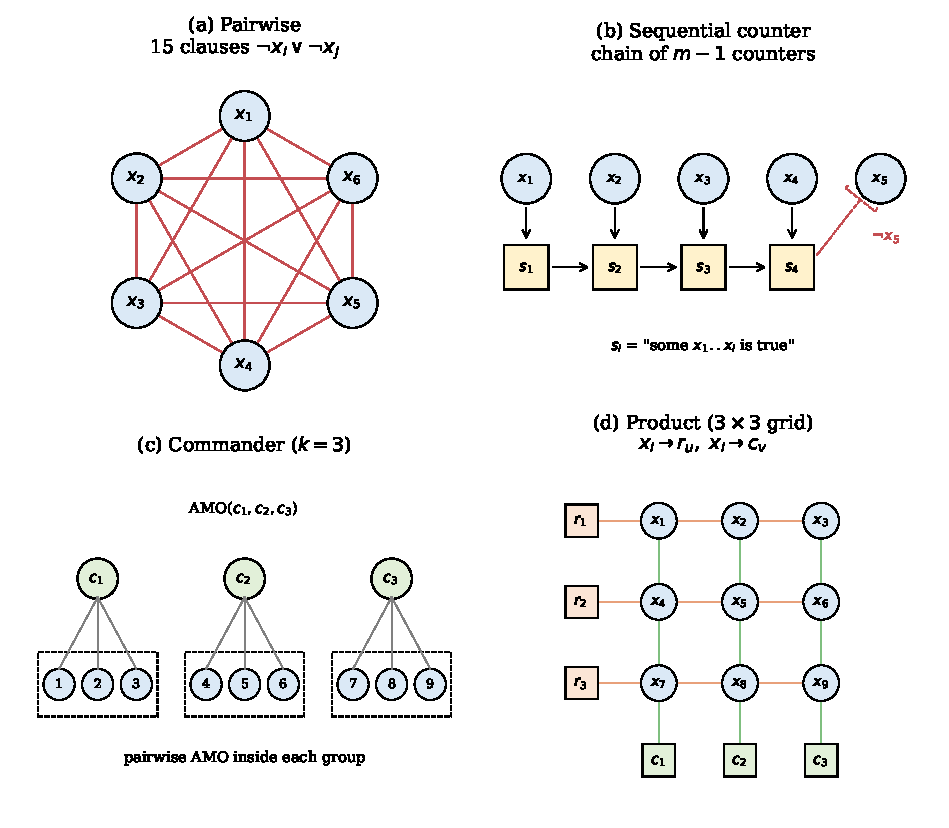
\includegraphics[width=0.8\linewidth]{figures/amo_encodings.pdf}
\caption{Structure of the AMO encodings. (a) Pairwise: one clause per pair (red edges). (b) Sequential counter: $x_i$ sets counter $s_i$, counters propagate to the right, and a set counter forbids later variables. (c) Commander: one commander per group of 3, AMO applied recursively to the commanders. (d) Product: each $x_i$ implies its row variable $r_u$ and column variable $c_v$; AMO is then applied to the rows and to the columns.}\label{fig:amo}
\end{figure}

\paragraph{Correctness.}
\begin{proposition}\label{prop:correct}
For each of the five encodings, an assignment of $x_1..x_m$ can be extended to the auxiliary variables so that all clauses are satisfied \emph{if and only if} at most one $x_i$ is true.
\end{proposition}
\noindent\textit{Proof sketch.} ($\Leftarrow$) If at most one $x_a$ is true, set the auxiliary variables ``honestly'': $y=$ code of $a$ (binary); $s_i=x_1\vee\dots\vee x_i$ (sequential); $c=\bigvee G$ (commander); $r_u, c_v$ true only for the cell of $x_a$ (product). Every clause is then satisfied. ($\Rightarrow$) Suppose $x_a$ and $x_b$ ($a<b$) are both true. \emph{Pairwise:} clause $(\neg x_a\vee\neg x_b)$ is violated. \emph{Binary:} the codes of $a$ and $b$ differ in some bit $j$, so $y_j$ would have to be both true and false. \emph{Sequential:} $x_a\Rightarrow s_a\Rightarrow s_{a+1}\Rightarrow\dots\Rightarrow s_{b-1}\Rightarrow\neg x_b$. \emph{Commander:} in the same group the pairwise clauses are violated; in different groups two commanders are true, which the recursive AMO forbids. \emph{Product:} two different cells differ in their row or column, so two row variables or two column variables are true, which the recursive AMO forbids. $\square$

We additionally checked Proposition~\ref{prop:correct} by brute force over all assignments for $m\le9$; the experimental check on the full N-Queens formulas is given in Section~\ref{sec:correct}.

\paragraph{Propagation strength.}
For a CDCL solver it is not enough that an encoding is correct; it should also let \emph{unit propagation} draw the obvious conclusions.
\begin{proposition}\label{prop:up}
In all five encodings, setting $x_a=1$ lets unit propagation alone derive $x_b=0$ for every $b\neq a$.
\end{proposition}
\noindent\textit{Proof sketch.} Pairwise: directly. Binary: $x_a$ fixes all $y_j$; for every $b\neq a$ some clause $(\neg x_b\vee\pm y_j)$ now has a false second literal. Sequential: forwards, $x_a\Rightarrow s_a\Rightarrow\dots\Rightarrow s_{m-1}$ and $s_{b-1}\Rightarrow\neg x_b$ for $b>a$; backwards, $(\neg s_{a-1}\vee\neg x_a)$ gives $\neg s_{a-1}$, then $(\neg s_{i-1}\vee s_i)$ gives $\neg s_{a-2},\dots,\neg s_1$, and $(\neg x_b\vee s_b)$ gives $\neg x_b$ for $b<a$. Commander and product: by induction over the recursion levels. $\square$

So no encoding is ``weaker'' than another in this sense. The encodings do differ in \emph{how many propagation steps} are needed. Table~\ref{tab:amo} reports the number of UP rounds needed to derive all $x_b=0$ after $x_a=1$ (worst case over $a$), which we call the \emph{propagation depth}. It is constant for pairwise and binary, grows logarithmically for commander and product, but grows \emph{linearly} for the sequential counter, whose information must travel along a chain of counter variables. We use this property in Section~\ref{sec:discussion} to explain the measured run times.

\begin{table}[pos=htbp]
\caption{Size and propagation depth of each AMO encoding over $m$ variables. The last columns give exact values for a line of $m=64$ variables (one row of the $64\times64$ board).}\label{tab:amo}
\centering
\begin{tabular}{llllrrr}
\toprule
 & & & & \multicolumn{3}{c}{$m=64$} \\
\cmidrule(lr){5-7}
Encoding & Aux.\ variables & Clauses & Prop.\ depth & Aux. & Clauses & Depth \\
\midrule
Pairwise           & $0$                    & $m(m-1)/2$             & $1$ & 0 & 2016 & 1 \\
Binary             & $\lceil\log_2 m\rceil$ & $m\lceil\log_2 m\rceil$ & $2$ & 6 & 384 & 2 \\
Sequential counter & $m-1$                  & $3m-4$                 & $\Theta(m)$ & 63 & 188 & 64 \\
Commander ($k=3$)  & $\approx m/2$          & $\approx 3.5m$         & $O(\log m)$ & 31 & 217 & 7 \\
Product            & $\approx 2\sqrt m$     & $\approx 2m+O(\sqrt m)$ & $O(\log\log m)$ & 28 & 172 & 5 \\
\bottomrule
\end{tabular}
\end{table}

\paragraph{PySAT built-in encodings.}
PySAT's \texttt{CardEnc.atmost(lits, bound=1, encoding=...)} offers several AMO encodings, of which we use four: \texttt{pairwise}; \texttt{seqcounter} (Sinz's sequential counter~\cite{sinz2005}); \texttt{bitwise} (the binary encoding~\cite{frisch2010}); and \texttt{ladder} (the ladder encoding of Gent and Nightingale~\cite{gent2004}, a chain of $m-1$ auxiliary variables closely related to the sequential counter). They serve as an independent reference for our own implementations (see \texttt{nqueens/encodings/pysat\_enc.py} in the accompanying repository).

%% ---------------------------------------------------------------------
\subsection{Constraint programming}
Let the integer variable $q_i\in\{0,\dots,N-1\}$ be the column of the queen in row $i$. Then ``one queen per row'' holds by construction, and the remaining constraints are~\cite{regin1994}:
\begin{equation}\label{eq:cp}
  \texttt{AllDifferent}(q_0,\dots,q_{N-1}),\quad
  \texttt{AllDifferent}(q_0+0,\dots,q_{N-1}+N-1),\quad
  \texttt{AllDifferent}(q_0-0,\dots,q_{N-1}-(N-1)).
\end{equation}
The first constraint covers columns, the second anti-diagonals and the third diagonals. Only $N$ variables are needed, compared with $N^2$ for SAT and ILP.

\paragraph{Why a global constraint helps.}
\texttt{AllDifferent} could be written as $\binom{N}{2}$ pairwise disequalities $q_i\neq q_j$, but these see only two variables at a time. Consider $q_0,q_1\in\{1,2\}$ and $q_2\in\{1,2,3\}$. No single disequality removes a value. The global constraint, however, notices that $q_0$ and $q_1$ use up the two values $\{1,2\}$ (a \emph{Hall set}~\cite{hall1935}), so $q_2=3$. R\'egin's algorithm~\cite{regin1994} finds all such deductions (generalised arc consistency) in polynomial time by computing a maximum matching between variables and values. This is the CP counterpart of choosing a strong AMO encoding in SAT: the whole line is reasoned about at once.

\paragraph{The two CP solvers.}
\emph{IBM CP Optimizer}~\cite{laborie2018} combines constraint propagation with tree search and restarts; its \texttt{AllDifferent} filtering strength is configurable. \emph{Google OR-Tools CP-SAT}~\cite{perron2024} is a \emph{lazy clause generation} solver~\cite{ohrimenko2009}: integer domains are represented by Boolean literals such as $[q_i=v]$ or $[q_i\le v]$, created on demand; every propagator explains its deductions as clauses, so that CDCL-style learning (Section~\ref{sec:cdcl}) also works on the CP model. In multi-threaded mode CP-SAT runs a portfolio of different strategies; here it runs with one worker. We test two CP-SAT models: the integer model of Eq.~\eqref{eq:cp} (``CP-SAT int'') and a Boolean model with $N^2$ variables, \texttt{AddExactlyOne} for rows/columns and \texttt{AddAtMostOne} for diagonals (``CP-SAT bool''), which mirrors the SAT model.

%% ---------------------------------------------------------------------
\subsection{Integer linear programming}
Let $x_{ij}\in\{0,1\}$ be 1 iff a queen is on $(i,j)$. The feasibility model is:
\begin{align}
  \textstyle\sum_{j} x_{ij} &= 1 && \forall i \quad\text{(rows)}\label{eq:ilp1}\\
  \textstyle\sum_{i} x_{ij} &= 1 && \forall j \quad\text{(columns)}\\
  \textstyle\sum_{(i,j)\in D} x_{ij} &\le 1 && \forall \text{ diagonal } D \text{ with } |D|\ge2.\label{eq:ilp3}
\end{align}
There is no objective: the solver stops at the first integer-feasible solution. The model has $N^2$ binary variables and $6N-6$ constraints (Eq.~\eqref{eq:lines}).

\paragraph{How branch-and-bound/cut solves it.}
The solver first solves the \emph{LP relaxation}, in which $0\le x_{ij}\le1$ may be fractional. If the LP solution is integral, it is a solution. Otherwise the solver strengthens the relaxation with \emph{cutting planes}, tries \emph{primal heuristics} (rounding, diving, local search) to find an integral point, and \emph{branches} on a fractional variable ($x_{ij}=0$ vs.\ $x_{ij}=1$), solving the two sub-problems recursively~\cite{wolsey1998}.

\paragraph{The LP relaxation is uninformative.}
Setting every $x_{ij}=1/N$ satisfies all constraints: each row and column sums to 1, and a diagonal of length $L\le N$ sums to $L/N\le1$. So the relaxation is always feasible and can return a ``uniform'' fractional point that says nothing about where queens should go. For N-Queens the work of an ILP solver therefore lies almost entirely in presolve, heuristics and branching, not in the LP bound. Note also that each diagonal inequality~\eqref{eq:ilp3} is already a \emph{clique inequality}, the strongest linear form of ``at most one''. It plays the same role as a compact AMO encoding: writing the same constraint as pairwise inequalities $x_a+x_b\le1$ would give a weaker relaxation and $\Theta(N^3)$ rows, just as pairwise does in SAT.

%% =====================================================================
\section{Methodology}\label{sec:method}
%% =====================================================================

\subsection{SAT model}
Let $x_{ij}$ (DIMACS index $iN+j+1$) be true iff a queen is on $(i,j)$. The CNF is:
\begin{align}
  &\textstyle\bigvee_j x_{ij}\;\wedge\;\mathrm{AMO}(x_{i0},\dots,x_{i,N-1}) && \forall i \quad\text{(rows)}\label{eq:sat1}\\
  &\textstyle\bigvee_i x_{ij}\;\wedge\;\mathrm{AMO}(x_{0j},\dots,x_{N-1,j}) && \forall j \quad\text{(columns)}\\
  &\mathrm{AMO}(\{x_{ij}: i-j=d\}),\;\mathrm{AMO}(\{x_{ij}: i+j=s\}) && \text{(diagonals of length}\ge2)\label{eq:sat3}
\end{align}
This gives $N^2$ main variables, $2N$ ALO clauses and $6N-6$ AMO constraints. Replacing ``AMO'' by any encoding of Section~\ref{sec:amo} gives one SAT variant. Auxiliary variables are numbered from $N^2+1$.

\paragraph{Closed-form CNF sizes.}
Using the line lengths of Eq.~\eqref{eq:lines} (rows and columns: $2N$ lines of length $N$; each diagonal direction: one line of length $N$ and two of each length $2,\dots,N-1$):
\begin{itemize}
  \item \emph{Pairwise.} $\sum_L\binom{|L|}{2} = 2N\binom{N}{2} + 2\Big[\binom{N}{2} + 2\sum_{\ell=2}^{N-1}\binom{\ell}{2}\Big] = N^2(N-1) + N(N-1) + 4\binom{N}{3} = \dfrac{N(N-1)(5N-1)}{3}$ AMO clauses, i.e.\ $\Theta(N^3)$.
  \item \emph{Sequential counter.} $\sum_L(3|L|-4) = 3(4N^2-4) - 4(6N-6) = 12(N-1)^2$ AMO clauses and $\sum_L(|L|-1) = 2(2N-1)(N-1)$ auxiliary variables, i.e.\ $\Theta(N^2)$.
  \item \emph{Binary, commander, product} likewise give $\Theta(N^2\log N)$, $\Theta(N^2)$ and $\Theta(N^2)$ clauses, respectively, by summing Table~\ref{tab:amo} over all lines.
\end{itemize}
The formulas match the implementation exactly (e.g.\ pairwise, $N=64$: $428{,}736+128=428{,}864$ clauses; sequential, $N=8$: $588+16=604$ clauses).

\subsection{Model size per paradigm}
Table~\ref{tab:modelsize} compares the three models. It also explains the licence limits observed later. Gurobi's community licence allows 2000 variables and CPLEX's 1000, so the $N^2$-variable ILP model fits only up to $N=44$ ($44^2=1936$) and $N=31$ ($31^2=961$). CP Optimizer's Community Edition limits the search space to about $2^{1000}$. If the search space is measured as the product of domain sizes, $N^N\le2^{1000}$, i.e.\ $N\log_2N\le1000$, which holds up to $N=140$. This is consistent with our observation that $N=128$ runs ($128\log_2128=896$) while $N=200$ is refused ($\approx1529$).

\begin{table}[pos=htbp]
\caption{Model size of each paradigm for an $N\times N$ board.}\label{tab:modelsize}
\centering\small
\setlength{\tabcolsep}{2.2pt}
\begin{tabular}{llll}
\toprule
Model & Variables & Constraints & Licence limit ($N_{\max}$) \\
\midrule
SAT (pairwise)            & $N^2$ Boolean             & $\Theta(N^3)$ clauses & none (open source) \\
SAT (other encodings)     & $N^2 + \Theta(N^2)$ aux.\ & $\Theta(N^2)$ / $\Theta(N^2\log N)$ clauses & none (open source) \\
CP int (CP-SAT, CPLEX)    & $N$ int, domain $N$       & 3 \texttt{AllDifferent} & CP-SAT: none; CPLEX: 128 \\
CP-SAT bool               & $N^2$ Boolean             & $2N$ ExactlyOne + $(4N-6)$ AMO & none (open source) \\
ILP (Gurobi, CPLEX MIP)   & $N^2$ binary              & $6N-6$ linear & Gurobi: 44; CPLEX: 31 \\
\bottomrule
\end{tabular}
\end{table}

\subsection{Solving procedure}
Algorithm~\ref{alg:sat} shows the SAT pipeline. Clauses are streamed directly into the solver's C/C++ clause database instead of first being stored as a Python list, which greatly reduces peak memory. Every returned solution, from any solver, is checked by the same independent validator.

\begin{algorithm}[htbp]
\caption{N-Queens via SAT}\label{alg:sat}
\begin{algorithmic}[1]
\Require board size $N$, AMO encoding \textit{enc}, SAT solver $S$
\Ensure a list of $N$ cells, or UNSAT
\State $S \gets$ new solver;\; $top \gets N^2$
\For{each line $L$ (row, column, diagonal, anti-diagonal) with $|L|\ge2$}
  \State $lits \gets \{x_{ij}:(i,j)\in L\}$
  \If{$L$ is a row or a column} \State add ALO clause $\bigvee lits$ \EndIf
  \State add the clauses of $\mathrm{AMO}_{enc}(lits)$ to $S$; update $top$
\EndFor
\If{$S.\mathrm{solve}()=$ SAT}
  \State $Q\gets\{(i,j): x_{ij}$ is true$\}$; check rows, columns, $i-j$, $i+j$ are all distinct
  \State \Return $Q$
\Else \State \Return UNSAT
\EndIf
\end{algorithmic}
\end{algorithm}

\subsection{Compared methods}
Fig.~\ref{fig:pipeline} gives an overview of the experimental pipeline.

\begin{figure}[pos=htbp]
\centering
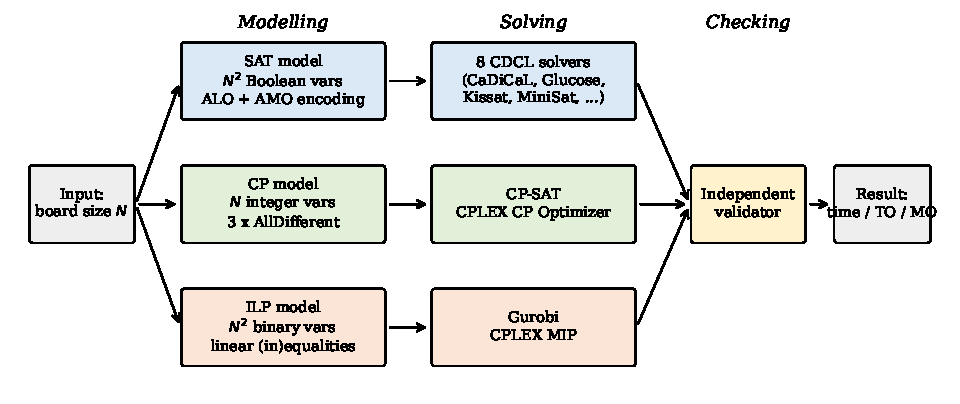
\includegraphics[width=\linewidth]{figures/pipeline.pdf}
\caption{Overview of the study: the same instance is modelled in three paradigms, solved by the corresponding solvers, and every solution is checked by one independent validator.}\label{fig:pipeline}
\end{figure}

Table~\ref{tab:methods} lists all methods.

\begin{table}[pos=htbp]
\caption{Methods compared in this study.}\label{tab:methods}
\centering
\begin{tabular}{llll}
\toprule
Paradigm & Solver / tool & Model & Variables \\
\midrule
SAT & 8 CDCL solvers (PySAT, pycryptosat) & CNF, Eqs.~\eqref{eq:sat1}--\eqref{eq:sat3} & $N^2$ Boolean + auxiliary \\
CP  & IBM CP Optimizer (CPLEX CP)          & \texttt{AllDifferent}, Eq.~\eqref{eq:cp} & $N$ integer \\
CP  & OR-Tools CP-SAT (int)                & \texttt{AllDifferent}, Eq.~\eqref{eq:cp} & $N$ integer \\
CP  & OR-Tools CP-SAT (bool)               & ExactlyOne / AtMostOne & $N^2$ Boolean \\
ILP & Gurobi                               & Eqs.~\eqref{eq:ilp1}--\eqref{eq:ilp3} & $N^2$ binary \\
ILP & CPLEX MIP                            & Eqs.~\eqref{eq:ilp1}--\eqref{eq:ilp3} & $N^2$ binary \\
\bottomrule
\end{tabular}
\end{table}

